% vim: set tw=78 tabstop=4 shiftwidth=4 aw ai:

\chapter{Proiectarea unui protocol Multiparty îmbunătățit în nucleul Linux}
\label{chapter:multiparty}

\section{Protocolul swift Multiparty}
\label{sec:multiparty:swift}

Protocolul \textit{swift} este un protocol multiparty generic de transport.
Scopul său principal este de a desemina conținut între peer-ii din swarm.
Practic răspunde la doar o singură cerere: \textit{'Uite aici hash-ul!
Dă-mi datele pentru el!}. Entități ca mediile de stocare, servere și
conexiuni sunt abstractizate și sunt invizibile la nivelul API-ului.
Dându-se un hash, datele sunt primite de la oricare sursă este dispoinibilă
și integritatea lor sunt verificate criptografic folosind arbori hash
Merkle \cite{merkle}.

Mare parte din facilitățile oferite de protocolul \textit{swift} sunt
definite de funcția sa de protocol de transport multiparty centrat pe
conținut. O diferență seminificativă între \textit{swift} și protocolul TCP
este faptul că TCP-ul nu deține nici o informație despre datele pe care le
transportă când datele sunt primite din user-space, pe când protocolul
\textit{switf} are date stabilite anterior și mulți peer-i participă la
distribuirea aceluiași set de date. Din acest motiv și din cauza faptului
ca pentru protocolul \textit{switf} ordinea recepționării informației are
puțină importanță, iar absența unui flux fiabil este componsată de redundanță,
renunță la abstractizarea TCP de livrare de flux de date fiabil secvenția.
Spre exemplu, datele ``out-of-order'' vor putea fi în continuare salvate și
aceeași piesă se poate obține de la alt peer

Principalul nostru obiectiv este integrarea protocolului \textit{swift} ca
un protocol de transport în stiva de rețea din nucleul Linux. Acest lucru
va crește semnificativ performanța transferurilor de date. Dorim să facem
acest lucru cu o intruziune minimă asupra nucleului Linux și modificând cât
mai puțin implementarea actuală de \textit{swift}. Un alt scop este de crea
un API transparent între nucleu și user-space. Un dezvoltator va folosi o
interfață de tip socket pentru a construi o aplicație peste protocolul
\textit{swift}. Pentru a îndeplini acest scop, am implementat un pas
intermediar. Am simulat bucata din kernel în user-space folosind socket-i
raw. Acest lucru are avantajul de a pune la dispoziție o metodă modulară de
a testa funcționalitățile.

\section{Proiectarea unui Protocol Multiparty}
\label{sec:multiparty:design}

În proiectarea sistemul nostru, am încercat diverse idei, fiecare cu
avantajele și dezavantajele ei. Vom prezenta unele dintre ideile
preliminare ce au condus la alegerea variantei finale.

Prima abordare la care ne-am gândit a fost să includem toate componentele
protocolului swift în nucleu. Acest lucru avea avantajul simplității și ar
fi însemnat un minim de schimbări în arhitectură. Implementarea actuală de
user space putea fi portată ca un modul de kernel.

Deși simplă, această abordare nu putea fi implementată din cauza
restricțiilor de mărime a memoriei în kernel. Pentru testulde integritate,
protocolul swift folosește arbore de hash Merkle. Păstarea acestui arbore
în memoria nucleului nu este scalabilă. Conținutul de pe Internet este mult
prea mare pentru a fi stocat în kernel space. Chiar dacă arborele reține
doar hash-urile datelor deseminate, spațiul tot este insuficient.

\section{Raw Socket Wrapper Implementation}
\label{sec:multiparty:raw-socket}

In figure Figure~\ref{fig:multiparty:architecture-overview} we see the main
conceptual modules: Application module, wrapper library, peer discovery
overlay and the swift transport protocol layer.

\begin{figure}
  \centering
  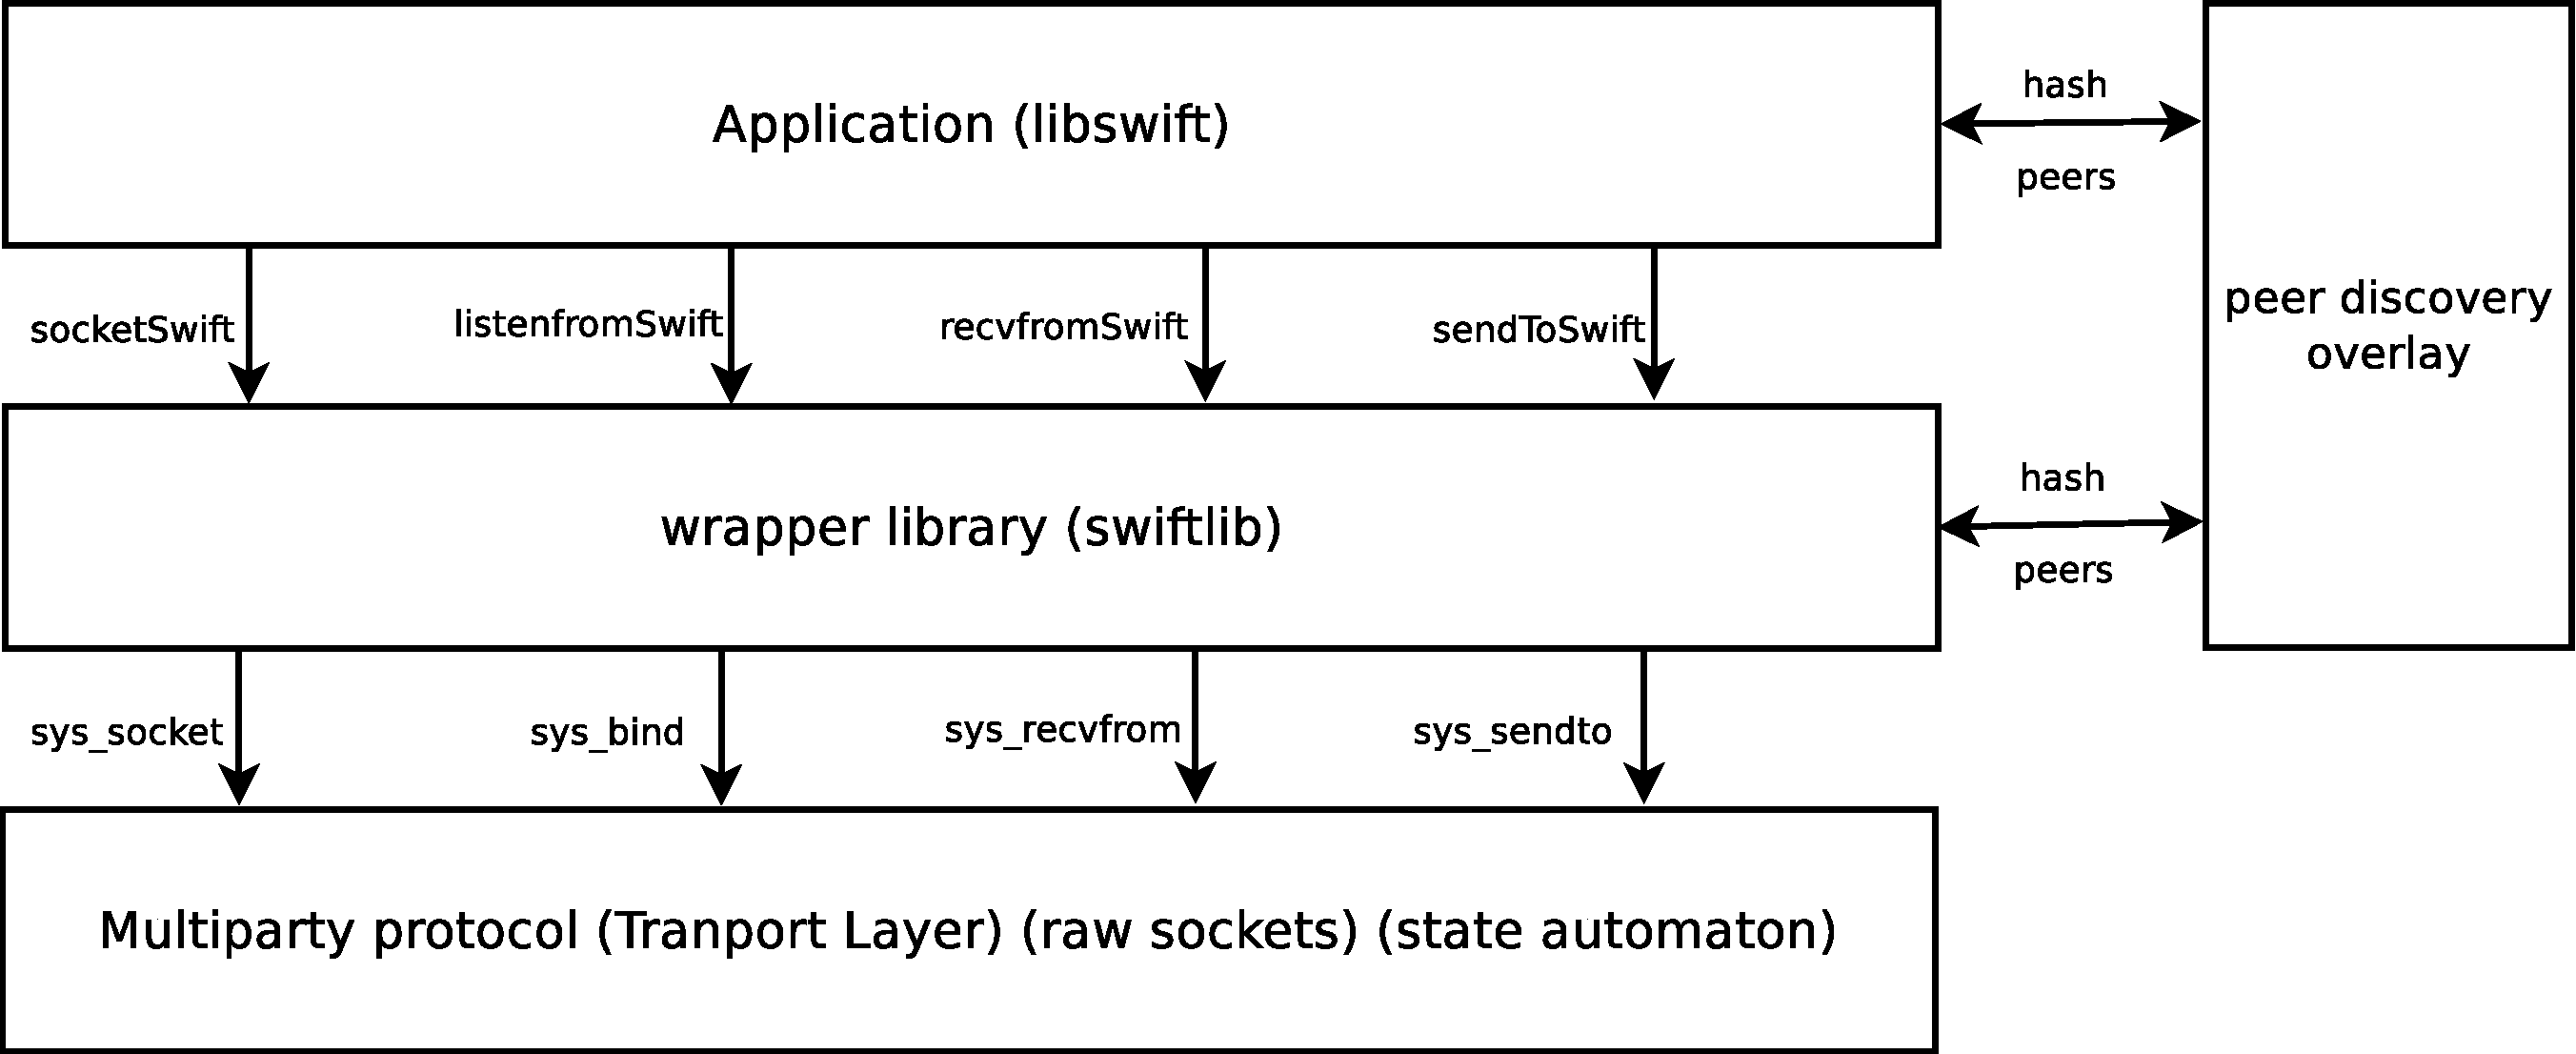
\includegraphics[width=0.6\textwidth]{src/img/multiparty/architecture-overview}
  \caption{Overview Architecture}
  \label{fig:multiparty:architecture-overview}
\end{figure}

The Application module represents the remaining part of the old swift
implementation. This is the part that remains in user space and contains the
file management and hash management features. 

The wrapper library module defines a socket-like API for the user space
applications. A regular program will use those calls instead of the normal
socket ones to use the multiparty sockets. For the moment those calls are
simulated system calls that initially are resolved with the socket raw
implementation (still in user space). In the future this wrapper library
will represent entry points into the kernel.

The peer discovery overlay will remain unchanged. It is still going to work
based on UDP sockets and link the same levels in the swift implementation as
before. The peer discover will be part of the application implementation and
it will be the developer's choice how to implement and how to manage it.

The multiparty protocol is implemented for now at user space level through a raw
socket layer to validate our architecture. This has the advantage of
simulating the real design modularization but also permits an easier debugging
and testing procedure of the integration. In the next step this part will be
represented by a kernel patch that will communicate through custom made system
calls with the wrapper library. This two phases are described in
Figure~\ref{fig:multiparty:detailed-architecture}.

\begin{figure}
  \centering
  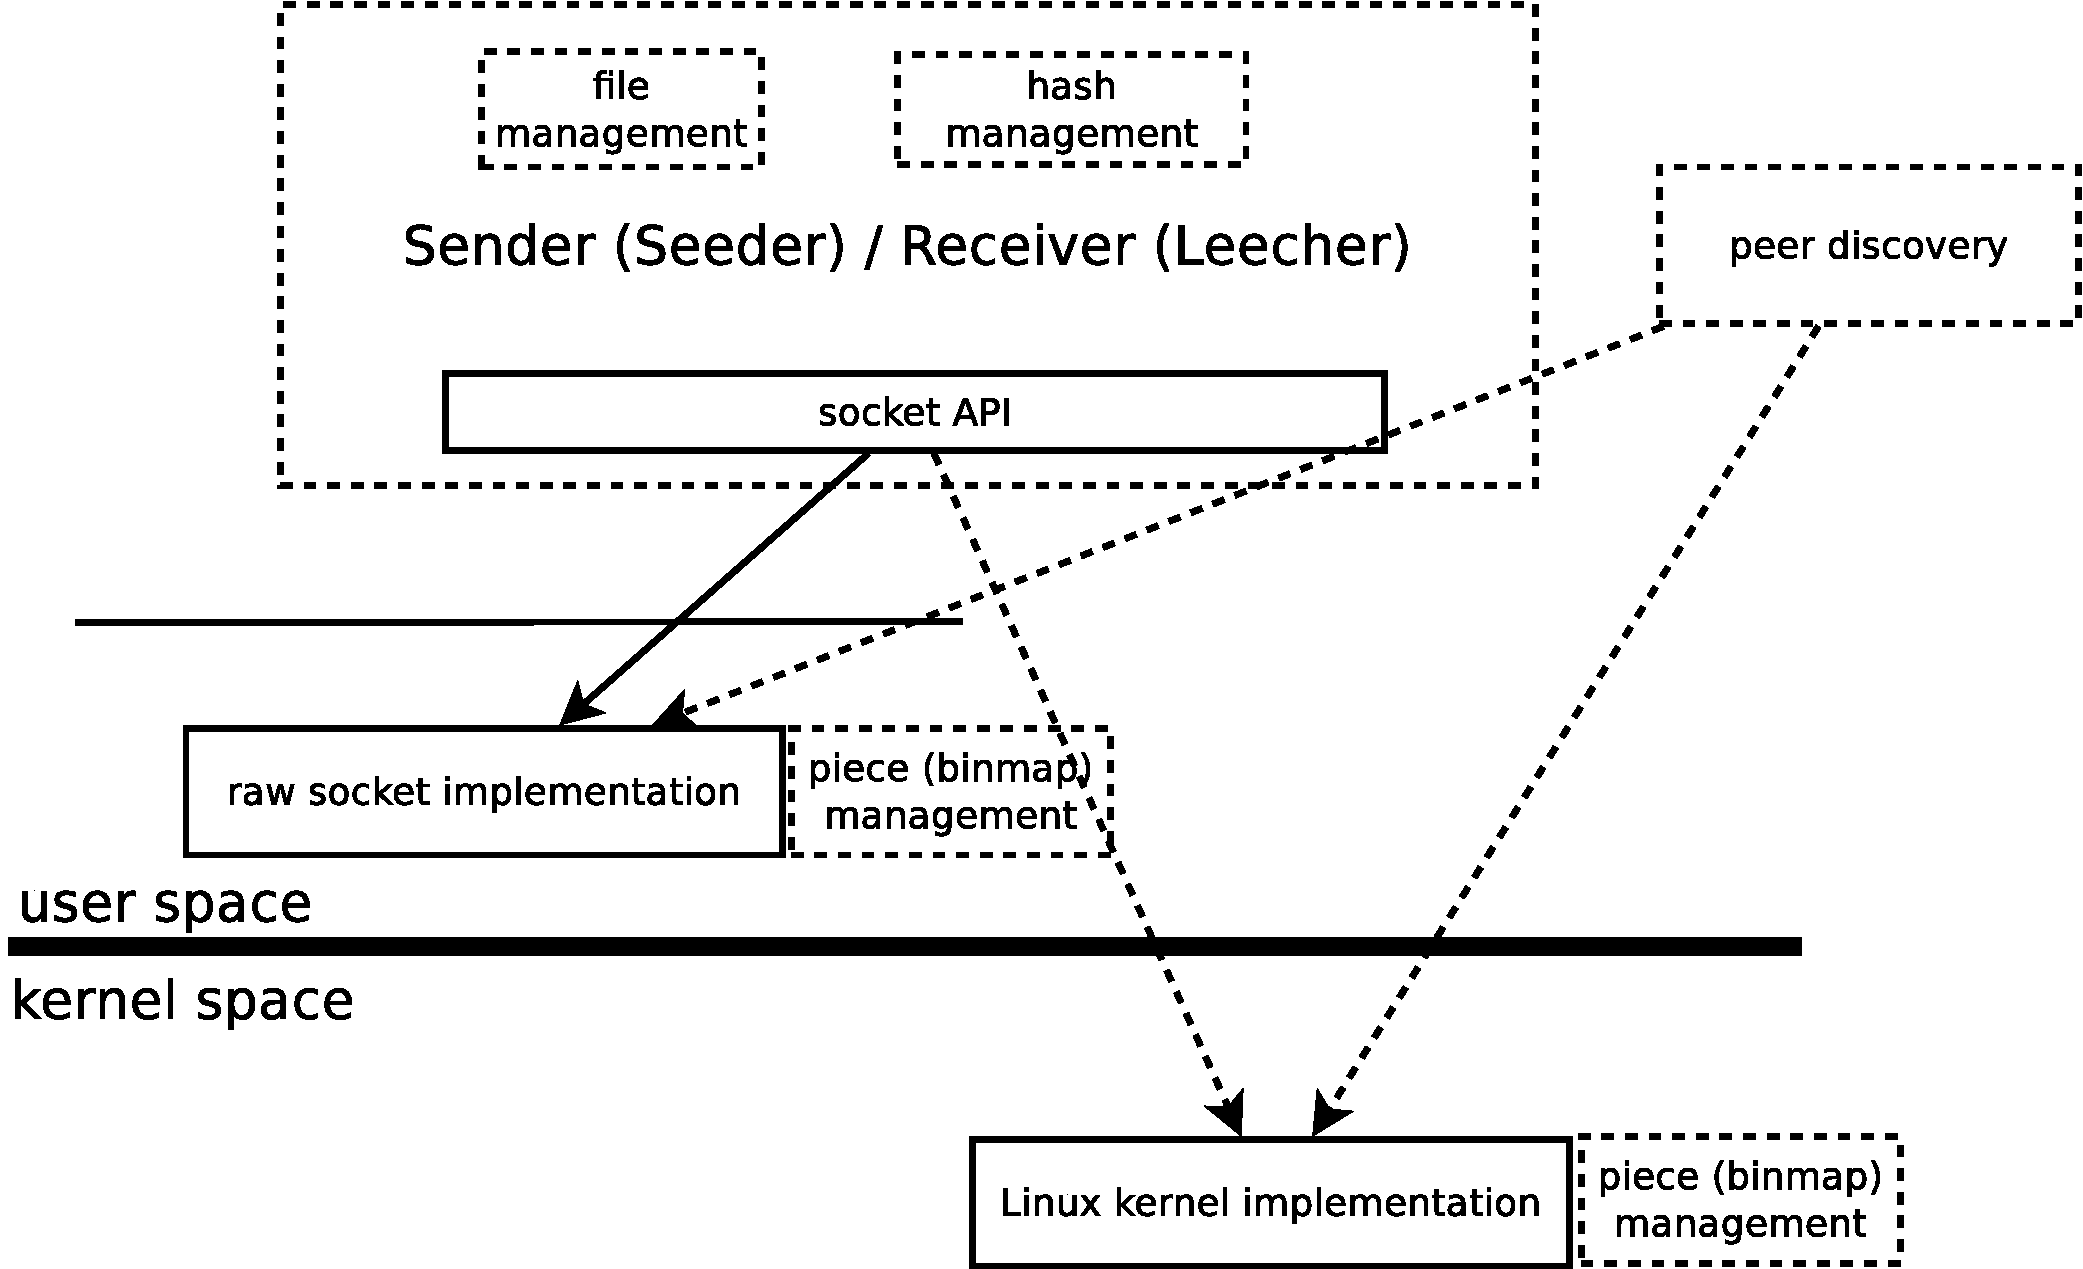
\includegraphics[width=0.6\textwidth]{src/img/multiparty/detailed-architecture}
  \caption{Detailed Architecture}
  \label{fig:multiparty:detailed-architecture}
\end{figure}

\begin{figure}
  \centering
  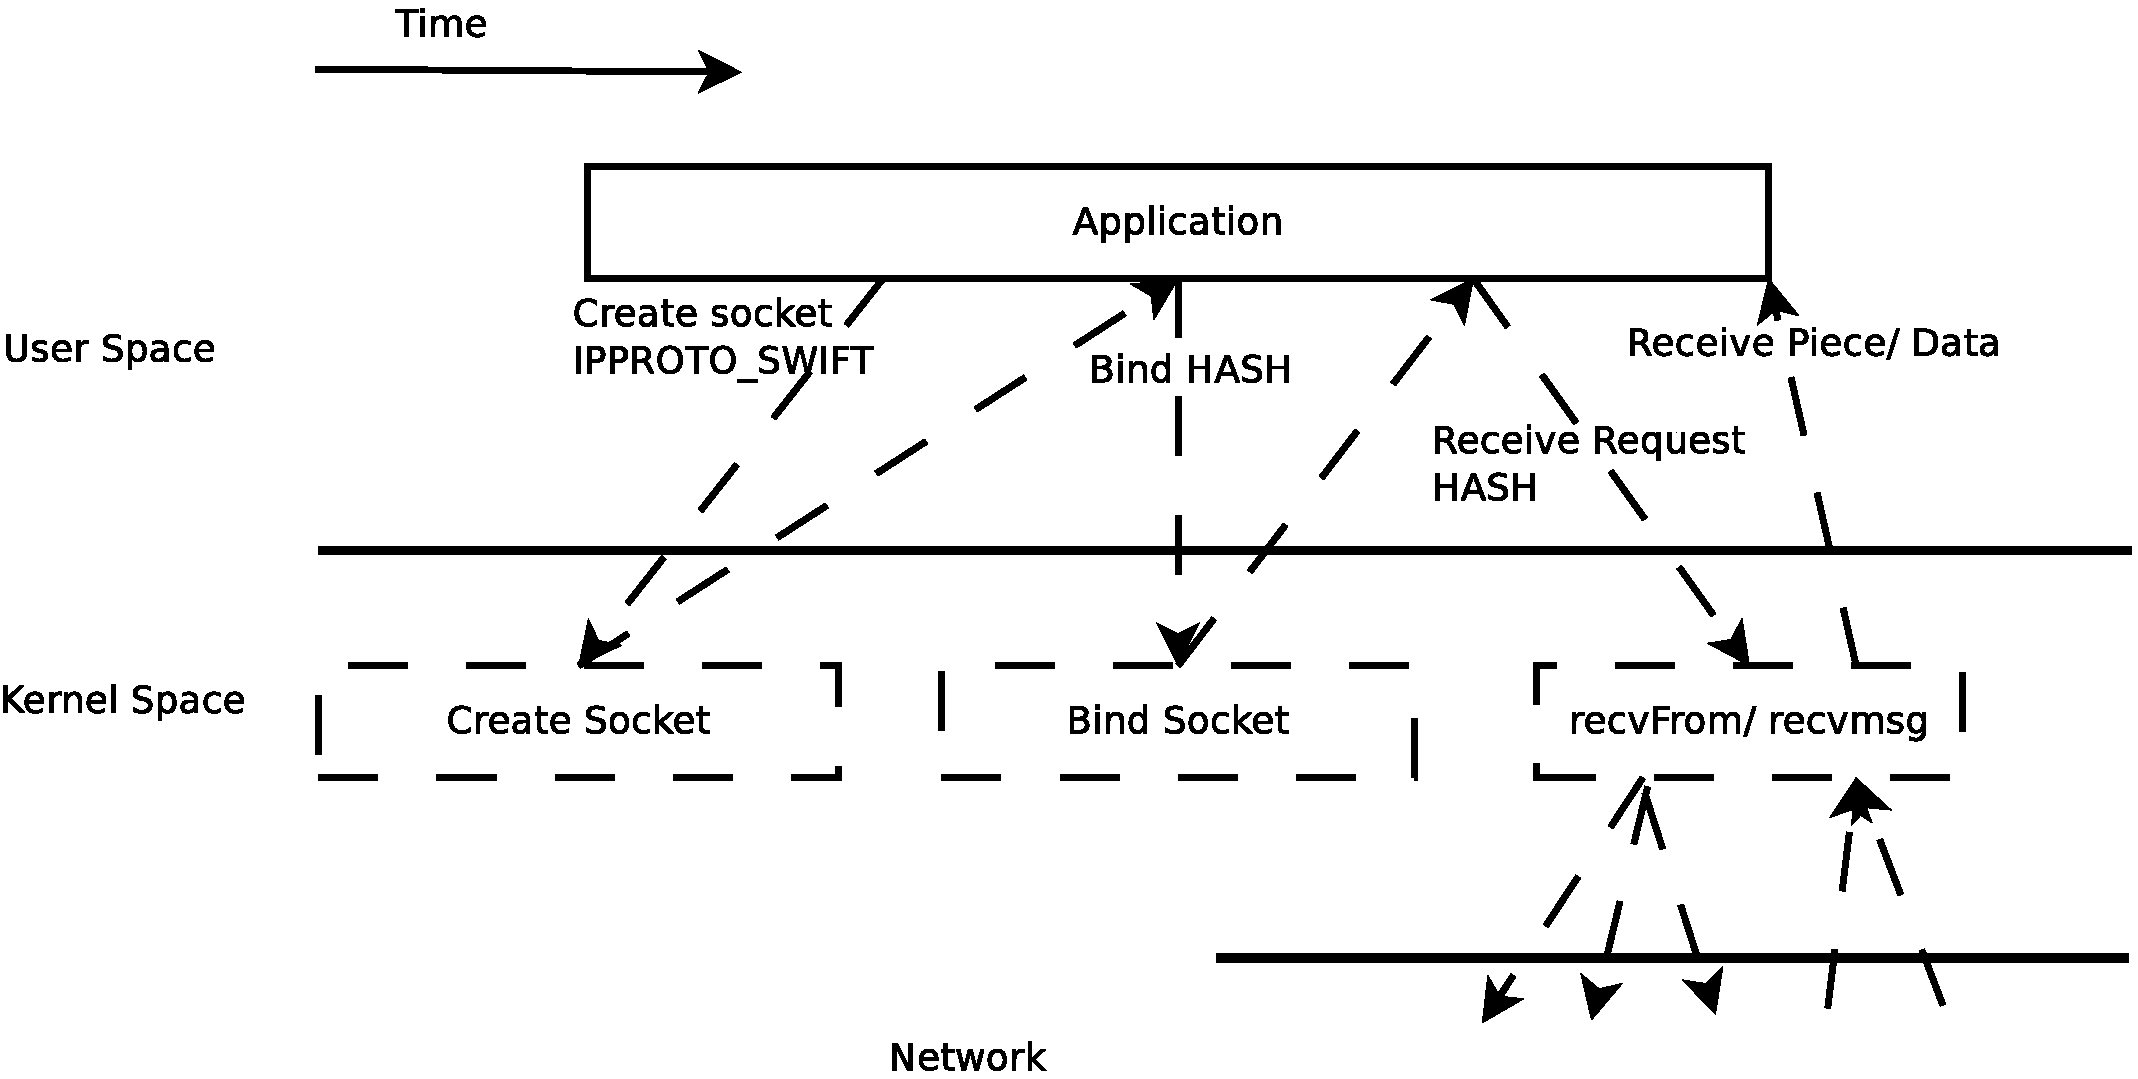
\includegraphics[width=0.55\textwidth]{src/img/multiparty/multiparty-recvmsg}
  \caption{Receiver Conceptual Model}
  \label{fig:multiparty:multiparty-recvmsg}
\end{figure}

Figure~\ref{fig:multiparty:multiparty-recvmsg} presents the conceptual model
of the Leecher. The Leecher is the one that requests data data. In order
to do this it must connect to the multiparty protocol by creating and binding
to a multiparty socket. When it binds to a socket, it uses the hash as a
parameter to find a connection with a peer that accesses the respective file.
This discovery is done through the separate peer discovery overlay. The
Leecher then waits for packets from seeders.

\begin{figure}
  \centering
  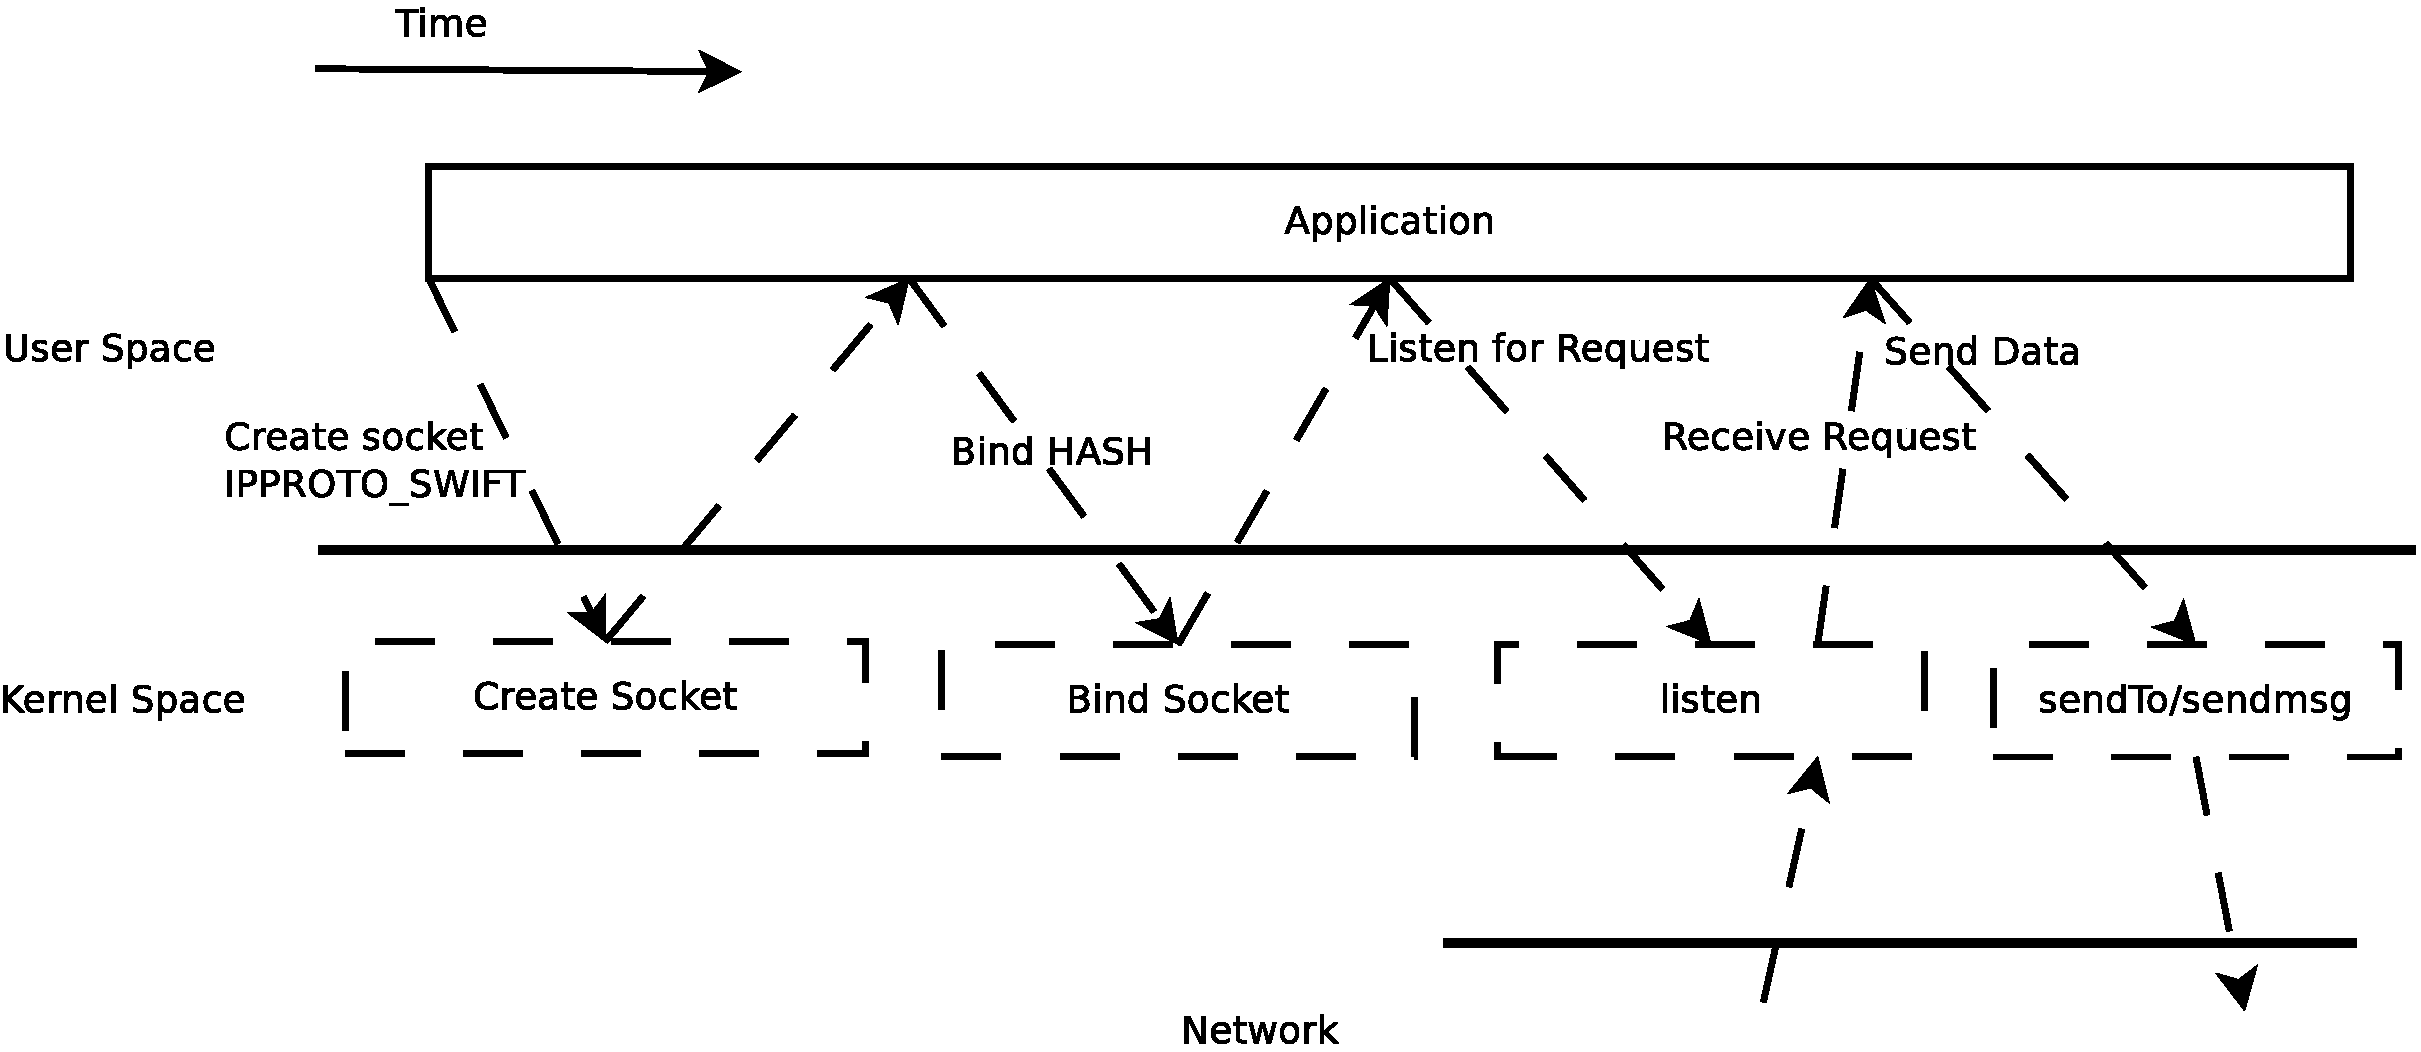
\includegraphics[width=0.55\textwidth]{src/img/multiparty/multiparty-sendmsg}
  \caption{Sender Conceptual Model}
  \label{fig:multiparty:multiparty-sendmsg}
\end{figure}

Figure~\ref{fig:multiparty:multiparty-sendmsg} presents the conceptual model
of the Seeder. The Seeder is the one that serves data to other Leechers. In
order to do this it must connect to the multiparty protocol by creating,
binding and listening to a multiparty socket. When binding, the Seeder
uses the hash as a parameter. This means that for every file hashed there will
be a socket on which the seeder that may receive and serve requests. The Seeder
then waits for requests and sends data packets as requested.

The  protocol is a generic multiparty transport protocol. Its mission is to
disseminate content among a swarm of peers.  Given a hash, the data is
received from whatever source available and data integrity is checked
cryptographically with Merkle hash trees. 

Our main focus when modifying the swift implementation is to have an impact on
time performance. With a communication protocol the greatest latency is
usually generated by waiting for the results from the network. The multiparty
communication model already takes care of this, so the next best thing is to
enhance the application time. We are doing this by decreasing time
penalties due to context switches between user space and kernel space. The
main idea is to reduce the number of system calls made from user space into
the kernel. This implicitly reduces the number of preemption moments.

The test suite is mainly implementing using arrays of function pointers or
function pointer structures. A top level structure defines test suites for
each function exported by the implementation. Each test suite is a series of
methods that test a variant of the call of the function.

\section{Kernel Framework for Multiparty Protocol Implementation}
\label{sec:multiparty:kernel-framework}

The introduction of a multiparty protocol in the Linux kernel was a challenge,
because of its particularities versus common protocol implementations. A
multiparty transport protocol uses multiple points in a communication, unlike
a traditional communication protocol that allows a sender endpoint and a
receiver endpoint.

In order to implement o transport protocol in the Linux kernel, several design
phases must be established:

\begin{itemize}
  \item Defining \texttt{IPPROTO\_\$\$}. This macro will identify the
  transport protocol. This will be subsequently used for creating a transport
  protocol socket.
  \item Defining a transport header. The framework we used defined two 8 bit
  ports, a source port and a destination port and a 16 bit lenght field. The
  latter field is the data length, including the tranport protocol header.
\end{itemize}

After the above have been completed, several data structures have to be
defined, as mentioned below.

A data structure that defines the new socket type. This is where we must save
information regarding the socket state, such as the destination or the source
port.
\begin{verbatim}
struct swift_sock {
    struct inet_sock sock;
    /* swift socket speciffic data */
    uint8_t src;
    uint8_t dst;
};
\end{verbatim}

The protocol definition, used by the socket, including its name and size are
defined in a \texttt{struct proto} structure.
\begin{verbatim}
static struct proto swift_prot = {
    .obj_size = sizeof(struct swift_sock),
    .owner = THIS_MODULE,
    .name = "SWIFT",
};
\end{verbatim}

The most important structure to be defined describes the operations that are
supported by a socket of a given type. For a datagram sending socket, the
implementation of \texttt{release}, \texttt{connect}, \texttt{sendmsg} and
\texttt{recvmsg} functions is sufficient.

The new packtets header are setup in the \texttt{net\_protocol} header. New
packets that are received directly from the network will fill the
\texttt{protocol} field in the IP header with the value of the implemented
Transport Level protocol.

Before compiling and inserting the module in the kernel, several socket
operations functions have to be filled; for swift (a datagram based protocol),
this would mean \texttt{release}, \texttt{bind}, \texttt{connect},
\texttt{sendmsg} and \texttt{recvmsg}. A handler for packets received from the
network must also be implemented. At protocol level, one must keep a mapping
between a port and a socket, meaning that the socket is bound to that port.

Unit tests have been employed for testing the protocol. Among those are a few
simple tests, to ensure basic functionality and then a set of new tests that
check error codes and protocol performance. Protocol performance is related to
ensuring scalability -- multiple simulateneous client connections.

Basic functional testing means the design and implementation of tests for each
function exposed by the protocol. That is, there is a given test for each of
\texttt{bind}, \texttt{connect}, \texttt{close}, \texttt{sendto},
\texttt{recvfrom}, \texttt{sendmsg}, \texttt{recvmsg}, \texttt{send} and
\texttt{recv}. The test suite is used is the same one used for the raw
socket implementation. Due to the identical API provided, we could easily use
those test for the kernel implementation.
